
\hwpart{I}{Understanding Your Data (10 points)}
Since the goal for generative modeling is to model the distribution of your data, it is important to first understand what does this distribution look like.

The dataset for this course is a custom subset of CelebA~\citep{liu2015faceattributes}, filtered to have specific properties. Your first task is to discover what those properties are.

\question{Visual Exploration}{5}

\subq{a}{2} Visualize a grid of at least 16 random samples from the training set. Include this grid below.

\answerbox{}{
\begin{center}
    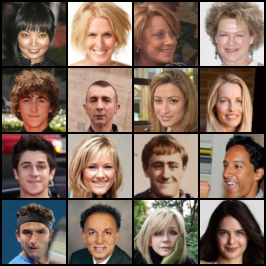
\includegraphics[width=0.55\textwidth]{figures/part_i_samples.png}
\end{center}
}
\includeanswer{q1a}

\subq{c}{3} This dataset was filtered from full CelebA using their 40 binary attributes. Based on your visual exploration, hypothesize which attributes were likely used to create this subset. What filtering criteria were used to create this subset? Why?

\answerbox{}{
From the sample grid, I do not think the subset is filtered to contain only one
specific demographic group. There are both male and female faces, multiple hair
colors, different ages, and different expressions. However, the images are
mostly clean, centered portraits with visible faces and little occlusion. My
hypothesis is that the filtering removed hard cases such as hats, glasses,
strong occlusions, extreme poses, or images where the face is not clearly
visible. The goal seems to be a cleaner face-generation subset rather than a
subset defined by a single semantic attribute.
}
\includeanswer{q1b}

\question{What did you learn?}{5}

\subq{a}{3} Imagine you found a pre-trained diffusion model that can reach SOTA performance on full CelebA (200K diverse faces). Now you generated samples and compared them to this filtered subset using KID or FID. Would you expect the FID and KID score to still be SOTA? Why?
\answerbox{}{
I would not necessarily expect the FID or KID score to remain SOTA. A
pre-trained model that performs well on full CelebA is trying to match the
broad distribution of all CelebA faces, which includes much more variation in
pose, occlusion, accessories, image quality, and facial attributes. This
filtered subset appears to be a narrower distribution of cleaner, centered,
less occluded face images.

FID and KID compare distributions of image features, not just whether each
generated image looks realistic by itself. Therefore, even high-quality samples
from a full-CelebA model may include valid CelebA faces that are outside the
filtered subset distribution. In that case, the generated distribution
$p_\theta(x)$ may be close to the full CelebA distribution but still mismatched
with the subset distribution, causing worse FID/KID scores against this subset.
}
\includeanswer{q2a}

\subq{b}{2} Based on your exploration, what kind of data augmentation transformation do you plan to use for your training and why?
\answerbox{}{
I plan to use only mild data augmentation, mainly random horizontal flipping.
The images are aligned face crops, and a horizontally flipped face should still
be a realistic sample from the same face distribution. This can increase the
effective diversity of the training data without changing the important facial
attributes too much.

I would avoid strong rotations, vertical flips, heavy cropping, or aggressive
color jitter. Those transformations could create unrealistic faces or shift the
training distribution away from the filtered CelebA subset that the diffusion
model is supposed to learn.
}
\includeanswer{q2b}

% ----------------------------------------------------------------------------
